\documentclass[letter,11pt]{article}

\usepackage[spanish,es-nodecimaldot]{babel}
\usepackage[utf8]{inputenc}

\usepackage{lmodern}
\usepackage[T1]{fontenc}
\usepackage{textcomp}

\usepackage{framed}
\usepackage[svgnames]{xcolor}
\colorlet{shadecolor}{Gainsboro!50}

\usepackage[labelfont=bf]{caption}
\usepackage{graphicx}
\usepackage{pstricks}
\usepackage{subcaption}

\usepackage{anysize}
\marginsize{3cm}{2cm}{2cm}{3cm}

\usepackage{url}
\usepackage{siunitx}
\usepackage{amsmath}
\usepackage{array}
\usepackage{alltt}

\usepackage{caption}
\newcommand{\source}[1]{\vspace{-11pt} \caption*{\small{\textbf{Nota:} {#1}}}}

\usepackage{fancyhdr}
\usepackage{lastpage}
\pagestyle{fancy}
\fancyhf{}
\fancyhead[LE,RO]{Laboratorio de Física Básica II}
\fancyfoot[CO,CE]{\thepage\ de \pageref{LastPage}}

\special{papersize=215.9mm,279.4mm}

\usepackage[
    pdfauthor={Carlos Eduardo Caballero Burgoa},%
    pdftitle={Laboratorio de Física Básica II},%
    pdfsubject={Ley de Boyle-Mariotte},%
    colorlinks,%
    citecolor=black,%
    filecolor=black,%
    linkcolor=black,%
    urlcolor=black,
    breaklinks]{hyperref}
\usepackage{breakurl}

\newcommand{\blankpage}{
\newpage
\thispagestyle{empty}
\mbox{}
\newpage
}

\renewcommand{\arraystretch}{1.2}

\title{Informe 8: Ley de \emph{Boyle}-\emph{Mariotte}}
\author{Carlos Eduardo Caballero Burgoa \\
    \small{\href{mailto:200201226@est.umss.edu}{200201226@est.umss.edu}}
}
\date{10 de julio de 2021}

\begin{document}

\maketitle
\begin{center}
    \textbf{Grupo}: J2 (Miércoles)\\
    \textbf{Docente}: Ing. Milka Mónica Torrico Troche\\
    \textbf{Carrera}: Ing. Electromecánica
\end{center}

\begin{abstract}
Este documento detalla el experimento realizado en simulador para hallar la
relación funcional entre la presión ($P$) y el ancho de un recipiente
contenedor ($x$) de un gas a temperatura ($T$), cantidad de materia ($n$), y
área transversal del contenedor ($A$) constantes, además del calculo de tal
área; para esto se realizó la medición de la presión en el contenedor a
diferentes variaciones del ancho del recipiente; posteriormente se calculó la
relación funcional con el método de mínimos cuadrados, finalmente se determinó
el valor del área transversal del contenedor, resultando ser:
$(356.74 \pm \num{2.27e-10}) [nm^2]; \num{6.36e-11}\%$.
\end{abstract}

\section{Introducción}

En el siglo XVII, \emph{Robert Boyle} estudió en forma sistemática y
cuantitativa el comportamiento de los gases. En una serie de experimentos,
\emph{Boyle} analizó la relación que existe entre la presión y el volumen de una
muestra de un gas. 

\begin{figure}
\begin{subfigure}{.30\textwidth}
    \centering
    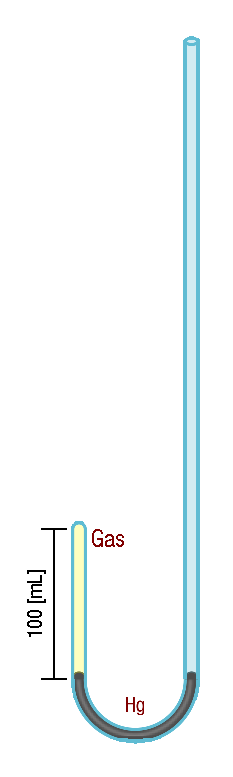
\includegraphics[width=0.75\textwidth]{resources/f1a.eps}
    \caption{Los niveles de mercurio son iguales y la presión del gas es igual a
    la presión atmosférica ($760 [mmHG]$). El volumen del gas es de $100 [mL]$.}
    \label{figura1a}
\end{subfigure}
\hfill
\begin{subfigure}{.30\textwidth}
    \centering
    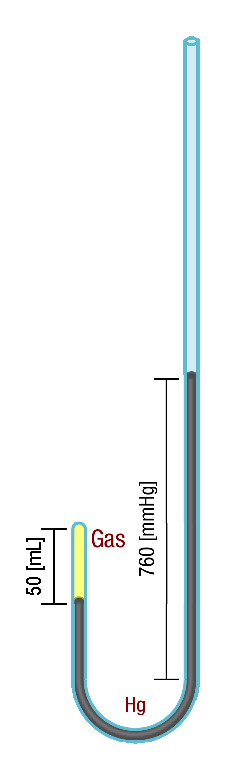
\includegraphics[width=0.75\textwidth]{resources/f1b.eps}
    \caption{Al duplicar la presión mediante la adición de mas mercurio, el
    volumen del gas se reduce a $50 [mL]$. \\
    }
    \label{figura1b}
\end{subfigure}
\hfill
\begin{subfigure}{.30\textwidth}
    \centering
    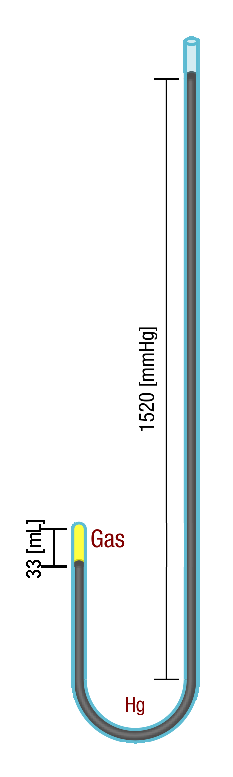
\includegraphics[width=0.75\textwidth]{resources/f1c.eps}
    \caption{Al triplicar la presión, el volumen del gas disminuye a un tercio
    del valor original. La temperatura y cantidad del gas se mantienen
    constantes.}
    \label{figura1c}
\end{subfigure}
\caption{Instrumento para el estudio de la relación \\
entre la presión y el volumen de un gas.}
\label{figura1}
\source{Química. (p. 180), \\
Chang, Raymond. 2010, McGraw-Hill.}
\end{figure}

El aparato que \emph{Boyle} utilizó en el experimento era muy sencillo (véase
\textbf{Figura \ref{figura1}}), En la \textbf{Figura \ref{figura1a}} la presión
ejercida sobre el gas es igual a la presión atmosférica y el volumen del gas es
de $100 [mL]$. (La parte superior del tubo se encuentra abierta y por tanto está
expuesta a la presión atmosférica.) En la \textbf{Figura \ref{figura1b}} se ha
añadido mas mercurio a fin de duplicar la presión sobre el gas, con lo que el
volumen del gas disminuye a $50 [mL]$. Al triplicar la presión sobre el gas su
volumen disminuye a un tercio de su valor original
(\textbf{Figura \ref{figura1c}}).

Es posible escribir una expresión matemática que muestre la relación hacia la
izquierda entre la presión y el volumen:

\begin{equation}
    P \propto \frac{1}{V}
\label{funcional1}
\end{equation}
\vspace{0.10cm}

Para cambiar esta proporcionalidad a una igualdad, se agrega un valor constante
$k_1$ llamado \emph{constante de proporcionalidad}:

\begin{equation}
    P = k_1\,\frac{1}{V}
\label{boyle1}
\end{equation}
\vspace{0.10cm}

La \textbf{Ecuación \ref{boyle1}} es una expresión matemática de la ley de
\emph{Boyle}, también se puede expresar como:

\begin{equation}
    PV = k_1
\label{boyle2}
\end{equation}
\vspace{0.10cm}

Esta forma de la ley de \emph{Boyle} establece que el producto de la presión y
el volumen de un gas a temperatura ($T$) y cantidad del gas ($n$) constantes, es
una constante \cite{Chang}.

Aunque los valores individuales de presión y volumen pueden variar mucho para
una muestra dada de un gas, siempre que la temperatura permanezca constante y la
cantidad de gas no cambie, $P$ multiplicada por $V$ siempre será igual a la
misma constante. Por consiguiente, para una muestra de una gas bajo dos
conjuntos de condiciones distintas a temperatura constante se tiene:

\begin{equation}
    P_1 V_1 = P_2 V_2
\label{boyle3}
\end{equation}
\vspace{0.10cm}

Conjuntamente a la ley de \emph{Boyle}-\emph{Mariotte}, existen otras leyes que
describen el comportamiento de los gases, estas son:

La ley de \emph{Charles}:

\begin{equation}
    V \propto T 
\label{charles}
\end{equation}
\vspace{0.10cm}

Donde la presión ($P$) y la cantidad de materia ($n$) son constantes.

Y la ley de \emph{Avogadro}:

\begin{equation}
    V \propto n 
\label{avogadro}
\end{equation}
\vspace{0.10cm}

Donde la presión ($P$) y la temperatura ($T$) son constantes.

Combinando las \textbf{Ecuaciones (\ref{boyle1}), (\ref{charles}) y 
(\ref{avogadro})}, se obtiene una ecuación maestra para el comportamiento de los
gases:

\begin{equation*}
    V \propto \frac{nT}{P}
\end{equation*}
\begin{equation*}
    V = R \frac{nT}{P}
\end{equation*}
\begin{equation}
    PV = nRT
\label{ideal}
\end{equation}
\vspace{0.10cm}

Donde $R$, la \emph{constante de proporcionalidad}, se denomina
\textbf{constante de los gases}. La \textbf{Ecuación \ref{ideal}}, conocida como
\textbf{ecuación del gas ideal}, explica la relación entre las cuatro variables
$P$, $V$, $T$ y $n$.

El valor de $R$ es:

\begin{equation*}
    R = \num{8.205746e-5} \left[\frac{m^3-atm}{K-mol}\right]
\end{equation*}
\vspace{0.10cm}

\section{Método experimental}

\begin{figure}
\centering
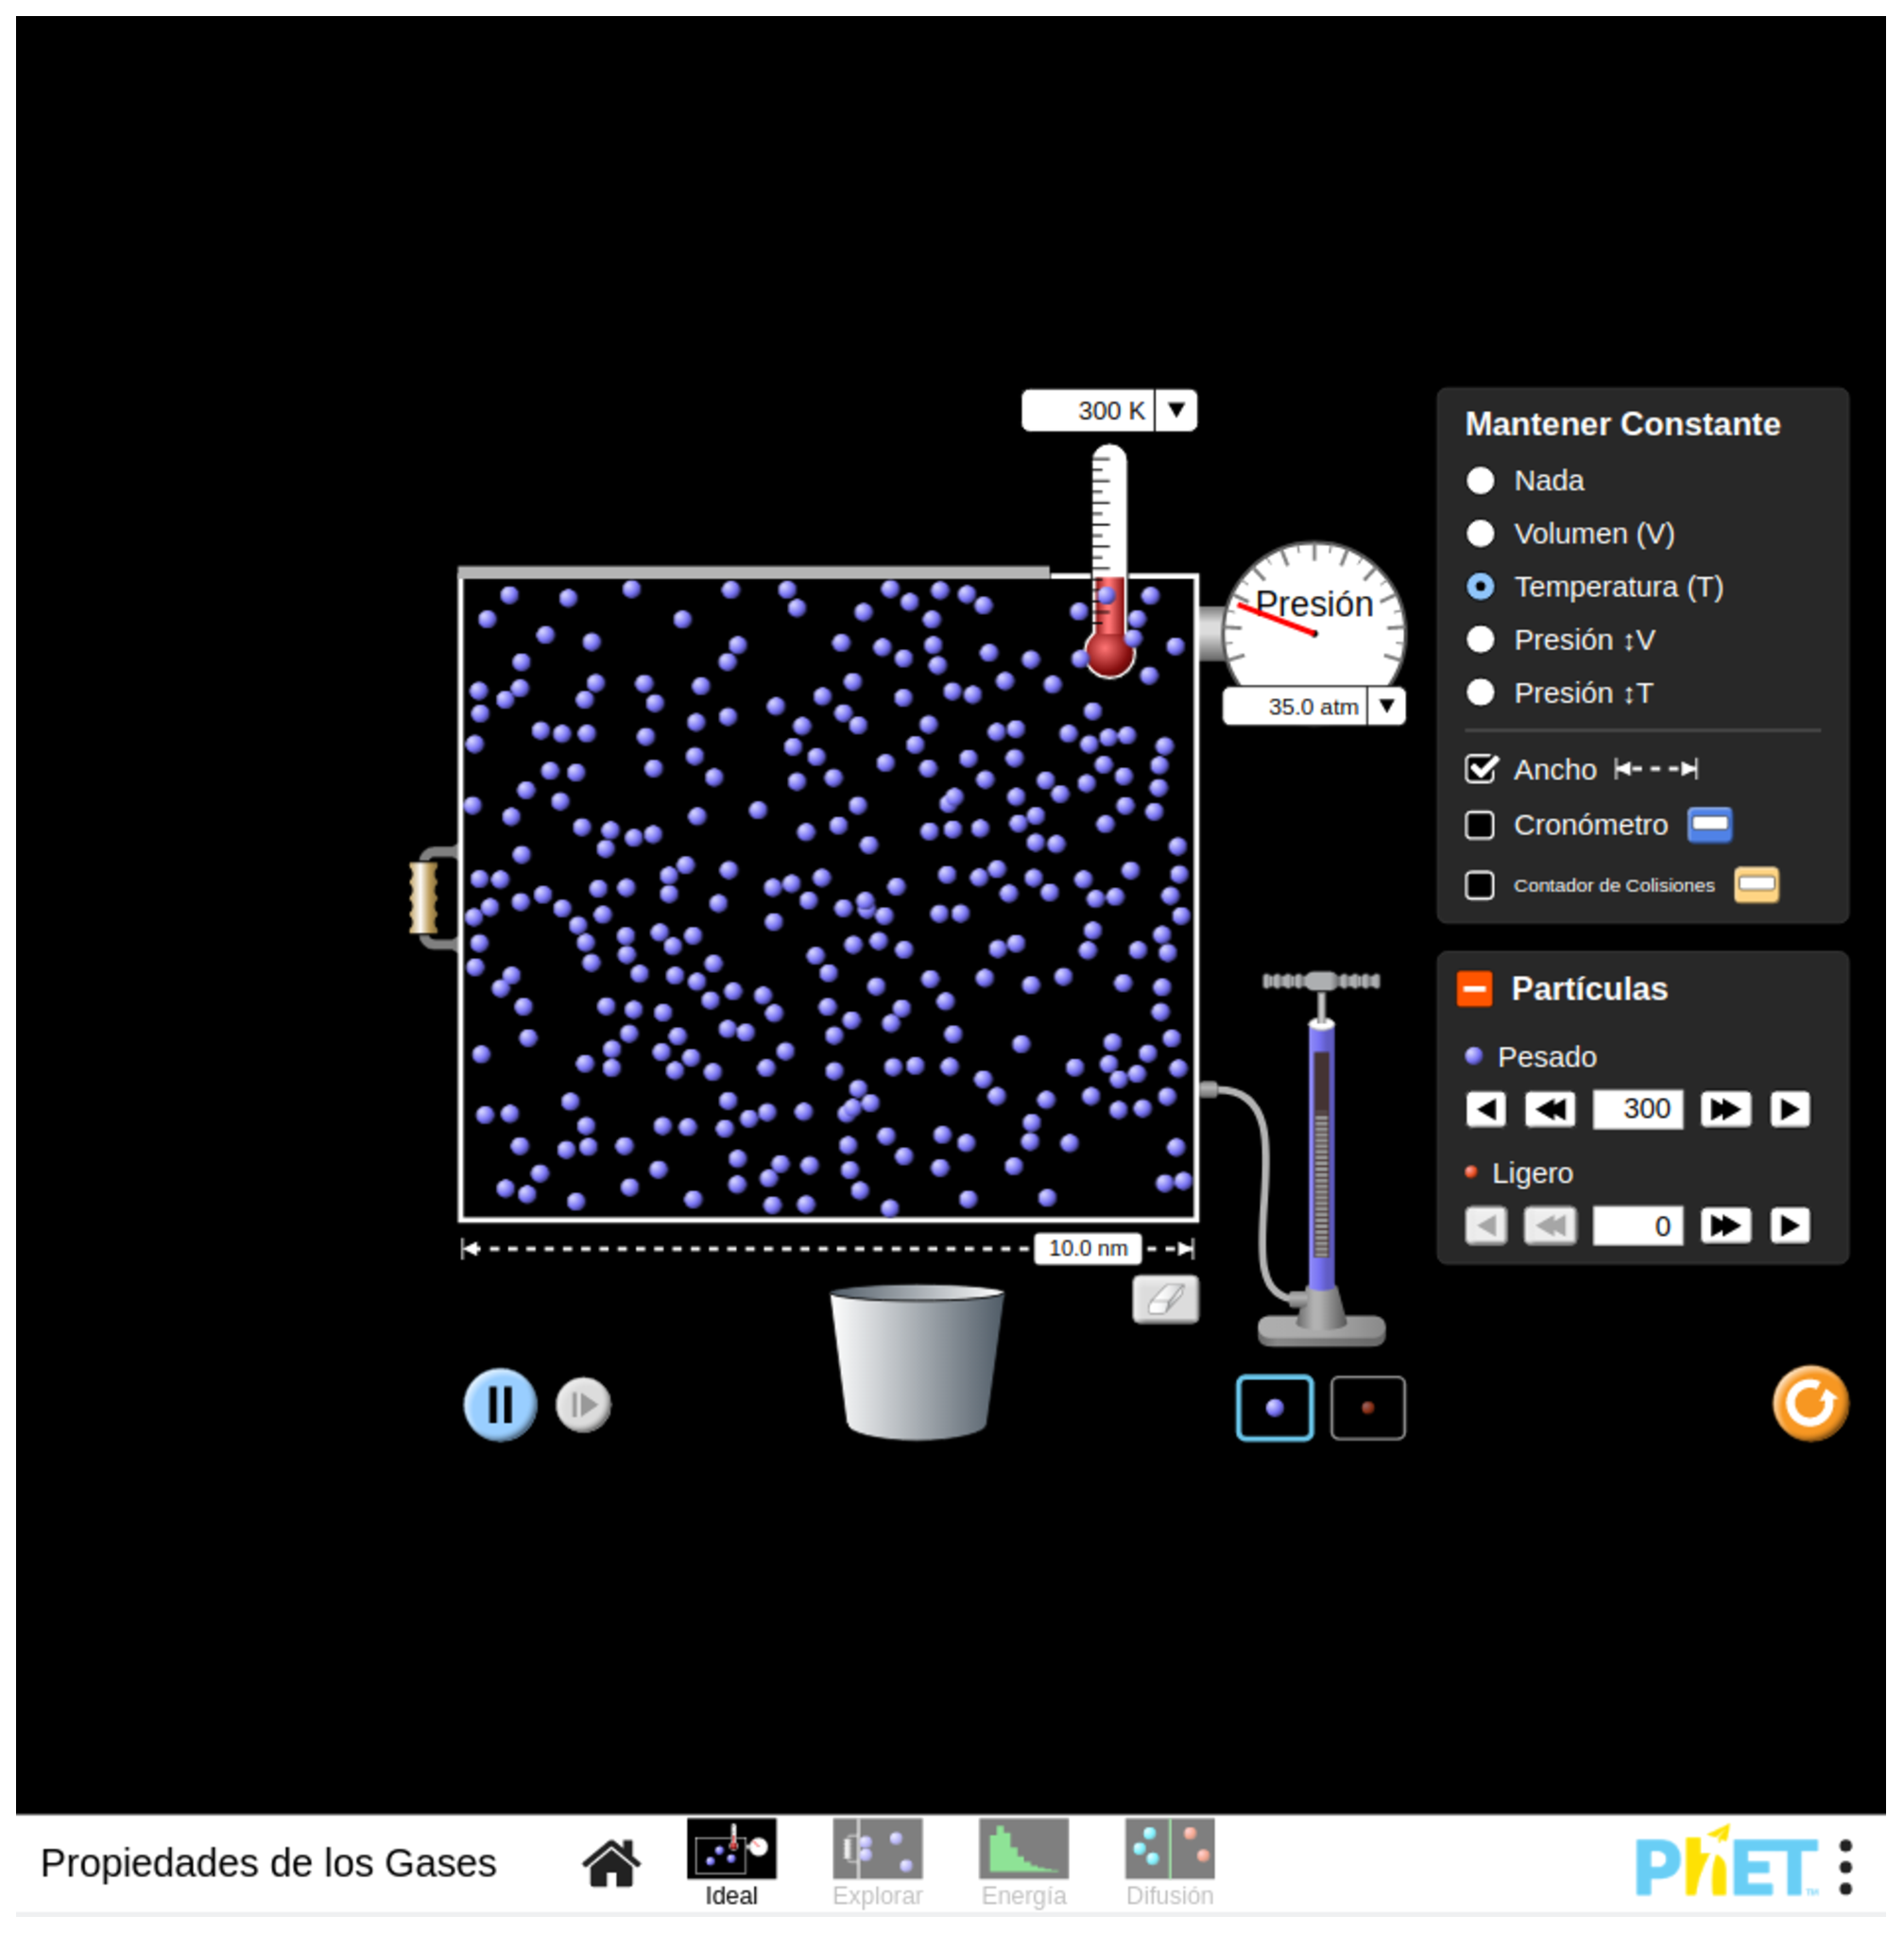
\includegraphics[width=0.95\textwidth]{resources/f2.eps}
\caption{Simulador de propiedades de los gases.}
\label{figura2}
\source{Captura propia.}
\end{figure}

Para la realización del experimento, se emplea el simulador \emph{PhET}
«Propiedades de los Gases», ubicado en la dirección web: \url{
https://phet.colorado.edu/sims/html/gas-properties/latest/gas-properties_es.html
}, tal como se presenta en la \textbf{Figura \ref{figura2}}.

A partir de la \textbf{Ecuación \ref{ideal}}, se obtiene:

\begin{equation*}
    P = nR\frac{T}{V}
\end{equation*}

Y asumiendo que el contenedor es rectangular, este será igual al área
transversal ($A$) por el ancho ($x$):

\begin{equation}
    P = nR\frac{T}{A x} = \left(nR \frac{T}{A}\right) \frac{1}{x}
\label{funcional2}
\end{equation}

Para el simulador, se registrarán diferentes valores del ancho del recipiente
($x$) y la variación de su presión ($P$)

Una vez medidos los datos, se procederá a graficar la relación ancho vs.
presión del recipiente, y con la ayuda del método de los mínimos cuadrados, se
halla la relación funcional entre las variables.

Finalizando con el calculo del valor del área transversal ($A$) del contenedor,
a partir de la \textbf{Ecuación \ref{funcional2}}:

\begin{equation*}
    k = nR \frac{T}{A}
\end{equation*}
\begin{equation}
    A = nR \frac{T}{k}
\label{area}
\end{equation}

Donde, la $n$, $T$ y $R$ son valores conocidos.
\\

\textbf{Datos necesarios para el experimento:} \\

Temperatura:

\begin{equation*}
    T = 300 [K]
\end{equation*}
\vspace{0.10cm}

Átomos dentro el contenedor:

\begin{equation*}
    N = 300 [\text{átomos}]
\end{equation*}
\vspace{0.10cm}

Numero de moles de gas, a partir del numero de \emph{Avogadro} ($N_A$):

\begin{equation*}
    N_A = \num{6.0221415e23}
\end{equation*}
\begin{equation*}
    n = \frac{N}{N_A} = \num{4.98162e-22} [moles]
\end{equation*}
\vspace{0.10cm}

\textbf{Datos tomados en el experimento:} \\

En el \textbf{Cuadro \ref{cuadro1}}, se pueden ver los valores tomados del 
experimento, tanto el ancho del recipiente, como la serie de mediciones de
presión, y su promedio.

\begin{table}[!h]
\begin{center}
\begin{tabular}{|c||>{\centering}m{1.4cm}<{\centering}|
                   |>{\centering}m{1.4cm}<{\centering}
                   |>{\centering}m{1.4cm}<{\centering}
                   |>{\centering}m{1.4cm}<{\centering}|
                   |>{\centering}m{1.4cm}<{\centering}|}
\hline
$i$ & $x_i [nm]$ &
    $P_{i1} [atm]$ & $P_{i2} [atm]$ & $P_{i3} [atm]$ & $\bar{P}_i [atm]$
    \tabularnewline \hline \hline
 1 & 15.0 & 23.6 & 23.0 & 23.8 & 23.4667 \tabularnewline \hline
 2 & 14.0 & 24.7 & 25.0 & 25.2 & 24.9667 \tabularnewline \hline
 3 & 13.0 & 26.6 & 27.3 & 26.9 & 26.9333 \tabularnewline \hline
 4 & 12.0 & 29.1 & 28.9 & 29.5 & 29.1667 \tabularnewline \hline
 5 & 11.0 & 32.0 & 31.8 & 31.6 & 31.8000 \tabularnewline \hline
 6 & 10.0 & 34.7 & 35.0 & 34.8 & 34.8333 \tabularnewline \hline
 7 &  9.0 & 38.8 & 39.0 & 39.2 & 39.0000 \tabularnewline \hline
 8 &  8.0 & 44.4 & 43.7 & 44.0 & 44.0333 \tabularnewline \hline
 9 &  7.0 & 50.0 & 50.5 & 50.4 & 50.3000 \tabularnewline \hline
10 &  6.0 & 58.5 & 58.3 & 58.7 & 58.5000 \tabularnewline \hline
11 &  5.0 & 69.8 & 69.9 & 70.0 & 69.9000 \tabularnewline \hline
\end{tabular}
\caption{Mediciones de presión en función del ancho del recipiente.}
\label{cuadro1}
\source{Elaboración propia.}
\end{center}
\end{table}

\section{Resultados}

\begin{figure}
\centering
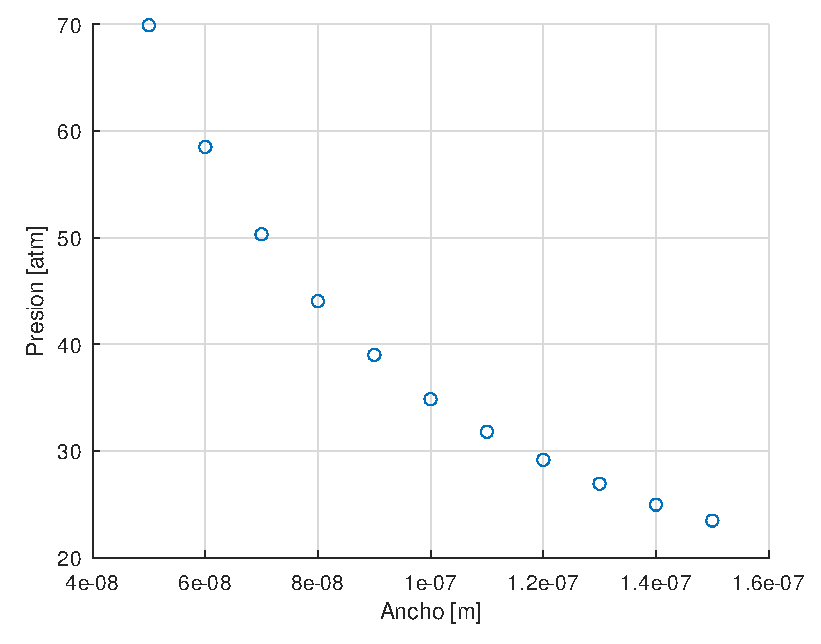
\includegraphics[width=0.75\textwidth]{resources/o1.1.eps}
\caption{Gráfica de ancho vs presión.}
\label{figura3}
\source{Elaboración propia.}
\end{figure}

A partir de los datos del \textbf{Cuadro \ref{cuadro1}} se genera la gráfica de
la \textbf{Figura \ref{figura3}}.

Posteriormente se linealizó la curva por medio de un cambio de variable, y se
calculó la recta de mejor ajuste por el método de los mínimos cuadrados,
resultando los siguientes valores:

\begin{equation*}
    A = (-12.58 \pm 0.05) [u]; 0.43\%
\end{equation*}
\begin{equation*}
    B = (-1.001 \pm 0.003) [u]; 0.33\%
\end{equation*}
\vspace{0.10cm}

Siendo su coeficiente de correlación ($r$):

\begin{equation*}
    r = -1.0000
\end{equation*}
\vspace{0.10cm}

Con los valores hallados, se calculan los valores originales de la curva,
resultando:

\begin{equation*}
    a = (\num{3.4376e-6} \pm \num{1.8489e-7}) [m-atm]; 5.38\%
\end{equation*}
\begin{equation*}
    b = (-1.001 \pm 0.003) [u]; 0.33\%
\end{equation*}
\vspace{0.10cm}

Resultando el modelo de ajuste:

\begin{equation*}
    P = 0.0000034\,x^{-1.00}
\end{equation*}
\vspace{0.10cm}

Por tanto la relación funcional entre $P$ y $x$, es:

\begin{center}
\begin{tabular}{|>{\centering}m{9.2cm}<{\centering}|}
\hline
\textbf{Resultado} 
\tabularnewline \hline
\\
$P \propto \dfrac{1}{x}$ \tabularnewline
\\
\hline
\end{tabular}
\end{center}
\vspace{0.10cm}

Verificándose el comportamiento establecido por la
\textbf{Ecuación \ref{funcional1}}.

Para el calculo de la área transversal del recipiente contenedor ($A$) se
utiliza la \textbf{Ecuación \ref{area}}, resultando:

\begin{center}
\begin{tabular}{|>{\centering}m{9.2cm}<{\centering}|}
\hline
\textbf{Resultado} 
\tabularnewline \hline
\\
$A = (356.74 \pm \num{2.27e-10}) [nm^2]; \num{6.36e-11}\%$ \tabularnewline
\\
\hline
\end{tabular}
\end{center}
\vspace{0.10cm}

\section{Discusión}

El simulador utilizado no provee información sobre la forma o dimensiones del
recipiente, permitiendo únicamente modificar el valor de una dimensión.

El resultado obtenido para el área transversal del recipiente resulto
$356.74 [nm]$, si se presupone una forma cuadrada, cada lado tendría un valor
de $18.89 [nm]$, que como puede verse en la \textbf{Figura \ref{figura2}} es
bastante razonable.

Otra particularidad sobre el simulador, es la cantidad de partículas que
utiliza, la cual no especifica claramente si hace referencia a átomos o
moléculas.

Se presupuso también que hace referencia a átomos, aunque seria mas lógico
pensar que son moléculas, pero sin saber el tipo de gas utilizado, no puede
hallarse la molaridad requerida en las ecuaciones utilizadas.

\section{Conclusiones}

Se halló la relación funcional entre el volumen (con área constante y ancho
variable) y la presión, confirmándose la \textbf{Ecuación \ref{boyle2}}.

También se calculó el valor del área transversal del recipiente con la ayuda
de la ecuación de los gases ideales (\textbf{Ecuación \ref{ideal}}).

\begin{thebibliography}{99}

\bibitem{Chang} Chang, Raymond. (2010).\\
Química.\\
10ma Edición.\\
Capitulo 5.

\bibitem{GUIA} Departamento de Física - UMSS.\\
Laboratorio de Física Básica II.\\
Guía - Cartilla de laboratorio.\\
Gestión I/2020.

\end{thebibliography}

\newpage
\section*{Apéndice A: Cálculos adicionales}

\subsection{Linealización de la curva}

En el \textbf{Cuadro \ref{cuadro2}}, se detallan los valores logaritmizados de
$x$ y $P$:

\begin{table}[!h]
\begin{center}
\begin{tabular}{|c||>{\centering}m{2.5cm}<{\centering}
                  |>{\centering}m{2.5cm}<{\centering}|}
\hline
$i$ & $ln(x_i)$ & $ln(P_i)$ \tabularnewline \hline \hline
 1 & -15.7126 & 3.1556 \tabularnewline \hline
 2 & -15.7816 & 3.2175 \tabularnewline \hline
 3 & -15.8557 & 3.2934 \tabularnewline \hline
 4 & -15.9358 & 3.3730 \tabularnewline \hline
 5 & -16.0228 & 3.4595 \tabularnewline \hline
 6 & -16.1181 & 3.5506 \tabularnewline \hline
 7 & -16.2235 & 3.6636 \tabularnewline \hline
 8 & -16.3412 & 3.7849 \tabularnewline \hline
 9 & -16.4748 & 3.9180 \tabularnewline \hline
10 & -16.6289 & 4.0690 \tabularnewline \hline
11 & -16.8112 & 4.2471 \tabularnewline \hline
\end{tabular}
\caption{Valores logaritmizados de $x$ y $P$.}
\label{cuadro2}
\source{Elaboración propia.}
\end{center}
\end{table}

\begin{figure}
\centering
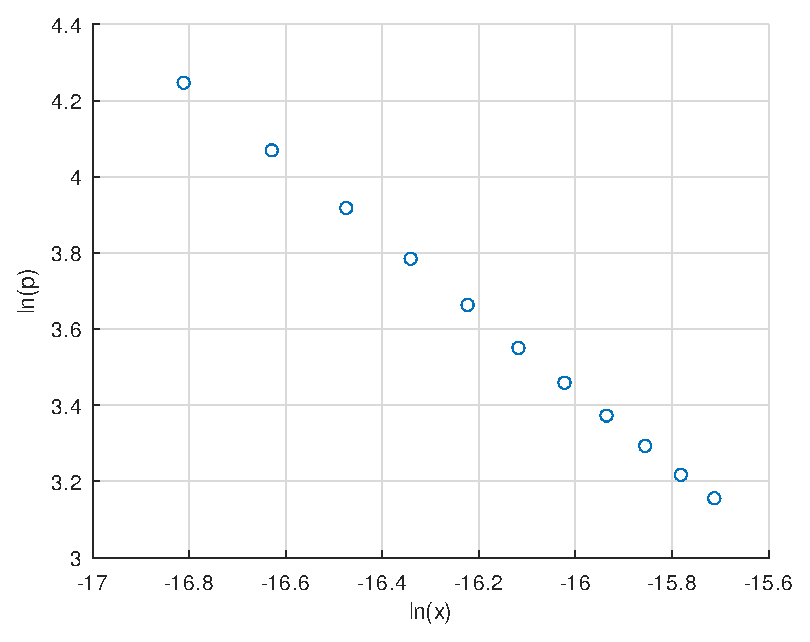
\includegraphics[width=0.75\textwidth]{resources/o1.2.eps}
\caption{Gráfica de $ln(L)$ vs. $ln(T)$.}
\label{figura4}
\source{Elaboración propia.}
\end{figure}

Los valores del \textbf{Cuadro \ref{cuadro2}}, pueden verse gráficamente en la
\textbf{Figura \ref{figura4}}.

\subsection{Método de mínimos cuadrados}

Se calculan los parámetros de la recta por el método de los mínimos cuadrados,
con la ayuda de los datos presentados en el \textbf{Cuadro \ref{cuadro3}}.

\begin{table}[!h]
\begin{center}
\begin{tabular}{|c||>{\centering}m{1.8cm}<{\centering}
                  |>{\centering}m{1.8cm}<{\centering}
                  |>{\centering}m{1.8cm}<{\centering}|
                  |>{\centering}m{1.8cm}<{\centering}
                  |>{\centering}m{1.8cm}<{\centering}
                  |>{\centering}m{2.1cm}<{\centering}|}
\hline
$i$ & $x^2_i$ & $y^2_i$ & $x_i y_i$ & $Y_i$ & $d_i$ & $d^2_i\,(\num{e-4})$
\tabularnewline \hline \hline
 1 & 246.8868 &  9.9577 & -49.5825 & 3.1508 &  0.0048 & 0.2292 \tabularnewline \hline
 2 & 249.0596 & 10.3526 & -50.7780 & 3.2199 & -0.0023 & 0.0542 \tabularnewline \hline
 3 & 251.4042 & 10.8463 & -52.2187 & 3.2941 & -0.0007 & 0.0049 \tabularnewline \hline
 4 & 253.9489 & 11.3773 & -53.7518 & 3.3742 & -0.0012 & 0.0139 \tabularnewline \hline
 5 & 256.7297 & 11.9679 & -55.4303 & 3.4613 & -0.0019 & 0.0344 \tabularnewline \hline
 6 & 259.7930 & 12.6066 & -57.2285 & 3.5567 & -0.0062 & 0.3809 \tabularnewline \hline
 7 & 263.2005 & 13.4217 & -59.4356 & 3.6622 &  0.0013 & 0.0176 \tabularnewline \hline
 8 & 267.0361 & 14.3258 & -61.8507 & 3.7802 &  0.0048 & 0.2293 \tabularnewline \hline
 9 & 271.4181 & 15.3508 & -64.5482 & 3.9139 &  0.0042 & 0.1726 \tabularnewline \hline
10 & 276.5210 & 16.5570 & -67.6635 & 4.0682 &  0.0008 & 0.0071 \tabularnewline \hline
11 & 282.6179 & 18.0376 & -71.3985 & 4.2507 & -0.0037 & 0.1341 \tabularnewline \hline
\end{tabular}
\caption{Valores para el método de mínimos cuadrados.}
\label{cuadro3}
\source{Elaboración propia.}
\end{center}
\end{table}

\begin{equation*}
    n = 11
\end{equation*}
\begin{equation*}
    \sum x_i = -177.9063
\end{equation*}
\begin{equation*}
    \sum y_i = 39.7322
\end{equation*}
\begin{equation*}
    \sum x^2_i = \num{2.8786e3}
\end{equation*}
\begin{equation*}
    \sum y^2_i = 144.8011
\end{equation*}
\begin{equation*}
    \sum x_i y_i = -64.8864
\end{equation*}
\begin{equation*}
    \Delta_1 = n \sum x^2_i - \left( \sum x_i \right)^2 = 14.1324
\end{equation*}
\begin{equation*}
    \Delta_2 = n \sum y^2_i - \left( \sum y_i \right)^2 = 14.1678
\end{equation*}
\begin{equation*}
    A = \frac{\sum y_i \sum x^2_i - \sum x_i y_i \sum x_i}{\Delta_1} = -12.5807
\end{equation*}
\begin{equation*}
    B = \frac{n \sum x_i y_i - \sum x_i \sum y_i}{\Delta_1} = -1.0012
\end{equation*}
\begin{equation*}
    \sum d^2 = \num{1.2782e-4}
\end{equation*}
\begin{equation*}
    \sigma^2 = \frac{\sum d^2_i}{n-2} = \num{1.4204e-5}
\end{equation*}
\begin{equation*}
    \sigma_A = \sqrt{\frac{\sigma^2 \sum x^2_i}{\Delta_1}} = 0.0538
\end{equation*}
\begin{equation*}
    \sigma_B = \sqrt{\frac{\sigma^2 n}{\Delta_1}} = 0.0033
\end{equation*}
\vspace{0.10cm}

Parámetros de la recta obtenida:

\begin{equation*}
    A = (-12.5807 \pm 0.0538) [u]; 0.4275 \%
\end{equation*}
\begin{equation*}
    B = (-1.0012 \pm 0.0033) [u]; 0.3321 \%
\end{equation*}
\vspace{0.10cm}

Siendo el coeficiente de correlación:

\begin{equation*}
    R = \frac{n \sum x_i y_i - (\sum x_i)(\sum y_i)}{\sqrt{\Delta_1 \Delta_2}}
      = -1.0000
\end{equation*}
\vspace{0.10cm}

La ecuación de la recta resultante es:

\begin{equation*}
    y = -12.5807 - 1.0012\,x
\end{equation*}
\vspace{0.10cm}

A partir de los parámetros de recta $A$ y $B$, se calculan los parámetros $a$ y
$b$ de la curva original y sus errores por el método de propagación de errores:

\begin{equation*}
    a = e^{A} = e^{-12.5807} = \num{3.4376e-6}
\end{equation*}
\begin{equation*}
    b = B = -1.0012
\end{equation*}
\begin{equation*}
    e_a = e^A e_A = e^{-12.5807}\,(0.0538) = \num{1.8489e-7}
\end{equation*}
\begin{equation*}
    e_b = e_B = 0.0033
\end{equation*}
\vspace{0.10cm}

Obteniendo finalmente los valores de la curva:

\begin{equation*}
    a = (\num{3.4376e-6} \pm \num{1.8489e-7}) [m-atm]; 5.3785\%
\end{equation*}
\begin{equation*}
    b = (-1.0012 \pm 0.0033) [u]; 0.3321\%
\end{equation*}
\vspace{0.10cm}

La ecuación de la curva resultante es:

\begin{equation*}
    P = a x^b = \num{3.4376e-6}\,x^{-1.0012} = 0.0000034\,\frac{1}{x}
\end{equation*}
\vspace{0.10cm}

\subsection{Calculo del área transversal}

Para el calculo del área transversal, se utiliza la \textbf{Ecuación \ref{area}}:

\begin{equation*}
    A = nR\frac{T}{a}
      = (\num{4.98e-22})(\num{8.2057e-5})\frac{300}{\num{3.4376e-6}}
      = \num{3.5674e-18} [m^2]
\end{equation*}
\vspace{0.10cm}

Y el error de la medición es:

\begin{equation*}
    \frac{\partial A}{\partial a} = -nR\frac{T}{a^2}
\end{equation*}
\begin{equation*}
    e_A = |-nR\frac{T}{a^2}| e_a = \num{2.2674e-30}
\end{equation*}
\vspace{0.10cm}

Resultando:

\begin{equation*}
    A = (\num{3.5674e-18} \pm \num{2.2674e-30}) [m^2]; \num{6.3560e-11}\%
\end{equation*}
\vspace{0.10cm}

\newpage
\section*{Apéndice B: Cálculos realizados en \emph{Octave}}

A continuación se presenta los cálculos realizados en el programa \emph{Octave}
para la generación de las gráficas, la linealización de la curva, el calculo
de los mínimos cuadrados y el valor del área transversal.

\begin{shaded}
\begin{alltt}
\footnotesize
\# Datos importados (i1.csv):
\input{resources/i1.csv}
\# Comandos ejecutados (o1.m):
\input{../../octave/graficar.m}
\input{../../octave/minimoscuadrados.m}
\input{resources/o1.m}
\# Salida del programa (o1.out):
\input{resources/o1.out}
\normalsize
\end{alltt}
\end{shaded}

\end{document}

